\chapter{The fractional graph shift operator and its applications}
\label{ch:FrGSO}

Over the last decade, theory and applications related to graph signal processing have been widely developed and attracted the attention of several scholars~\cite{ortega2018,richard2018,ribeiro2018}. The reader may recall from Chapter \ref{ch:reviewGSP} that GSP aims to extend concepts and operations of classical digital signal processing to scenarios in which the signals lie over irregular domains. Such scenarios include, for instance, sensors arbitrarily positioned in a geographic region and measuring some climatological variable, points of a three-dimensional cloud representing some virtual object and its attributes, people linked according to their interests and proximity relationships in a social network and so on~\cite{chen2014,zhang2014,benzi2016,weiyu2018,saad2018,jiang2021,gama2019,liu2019,zhang2020,ferreira2020,zhang2021,xiao2021,sun2021}.

Among the research fronts active in GSP, the one that investigates alternatives to the shift operators, employed as building blocks to describe graph signals and systems, deserves to be highlighted~\cite{girault2015translation,gavili2017,fan20191,fan2019,mollaebrahim2021,shafipour2018,shafipour2019}. {In fact, when the purpose is to consider linear operators in this context, any matrix can be chosen to play the role of elementary building block; multiplying a matrix by a graph signal represented as a vector produces another signal whose samples result from a linear combination of the samples of the original signal. In this scope,} the use of matrices other than the \textit{standard} adjacency matrix and the Laplacian for the mentioned purpose may {be more suitable in specific scenarios and to carry out specific (graph) signal processing tasks. Even when the focus is on designing other graph operators (e.g., the graph Fourier transform), the decision about which elementary operator to use has an impact on the expected results.}

    {Regarding the issue discussed in the last paragraph, some works archived in the GSP literature can be brought to the fore. In~\cite{girault2015translation}, for example, the authors propose an isometric graph translation operator that is described in the spectral domain as a phase shifting operator; this operator shares key properties with the time shift and behaves reasonably in the vertex domain. In~\cite{gavili2017}, the authors define an energy-preserving shift operator that satisfy many properties similar to their counterparts in classical signal processing; the GSP framework based on the referred operator enables the signal analysis along a correlation structure defined by a graph shift manifold. In~\cite{fan20191} and~\cite{fan2019}, the authors employ different features associated with a graph to generate a series of shift operators and design a graph-filter-based classifier. Although the proposed method produces better results than those achieved using conventional graph-filter-based classifiers, it requires dealing with a non-convex optimization problem whose solution involves a relatively high computational cost. In~\cite{mollaebrahim2021}, motivated by the typical scenario of asymmetric communications in wireless sensor networks, the authors study the optimal design of graph shift operators to perform decentralized subspace projection for asymmetric topologies. Obtaining the referred operators can be performed either by solving an optimization problem or by employing a decentralized algorithm based on an Alternating Direction Method of Multipliers (ADMM). In~\cite{shafipour2018} and~\cite{shafipour2019}, the goal is to construct a graph Fourier transform for directed graphs (digraphs), such that the corresponding orthonormal frequency components are as spread as possible in the graph spectral domain. The method uses the Laplacian of an undirected version of the digraph and involves non-convex, orthonormality-constrained optimization problems.}

    {This chapter brings contributions related to the above mentioned works by discussing the} possibility (and potentially useful consequences) of {computing} a non-integer power $\mathbf{A}^a$, $a\in\mathbb{R}$, of the adjacency matrix $\mathbf{A}$, {which is taken as} the (unit) graph shift operator~\cite{sandryhaila2014big}. {As a consequence}, the notion of fractional shift (or delay) of signals on graphs is presented, {which, to the best of the author's knowledge, has not yet been addressed in the literature. Differently from the referred papers, in which new operators are created or standard operators are adjusted using strategies potentially expensive from the computational point of view, a relatively simple generalization is proposed, which fills a theoretical gap concerning the extension to the GSP framework of a well-established concept in the classical signal processing.}

This chapter contains mostly the content of the paper \cite{ribeiro2022fractional}, published on the IEEE Access journal, and presents the contributions listed below.
\vspace{-1em}
\begin{itemize}[noitemsep]
    \item The introduction of the fractional graph shift operator $\mathbf{A}^a$ and the discussion of its several aspects. More specifically, the demonstration that $\mathbf{A}^a$ can be computed by using the theory of matrix functions, considering the Jordan decomposition of $\mathbf{A}$.

    \item The demonstration that $\mathbf{A}^a$ acts as a graph filter, furthermore giving its frequency response and discussing issues related to fractionally shifting graph signals containing descontinuities (Gibbs phenomenon).

    \item An analogy between the proposed graph fractional operator and that considered in the classical discrete-time case; suggesting that, when a directed ring graph with $N$ vertices is considered, the response of the corresponding graph filter related to $\mathbf{A}^a$ converges to that of the classical fractional delay filter as $N$ grows.

    \item The determination of the polynomial representation of $\mathbf{A}^a$ and, with that, the demonstration that, for any graph, such an operator can be implemented as a linear and shift-invariant (LSI) graph filter.
\end{itemize}

This chapter is organized as follows. In Section~\ref{sec:fracshift}, it is introduced the concept of fractional shift on graphs and the main contributions are developed: the computation of $\mathbf{A}^a$ in Subsection~\ref{subsec:comp}, discussion of its interpretation in Subsection~\ref{subsec:interpret}, demonstration of its consistency with the ideal fractional delay filter in Subsection~\ref{subsec:consist} and determination of its polynomial representation in Subsection~\ref{subsec:poly}. Section~\ref{sec:num} is devoted to numerical results related to the developed theory: it is firstly presented a small example regarding the polynomial representation of $\mathbf{A}^a$ in Subsection~\ref{subsec:num1}; then a real-world graph signal is considered (temperature measured by weather stations) and it is demonstrated that, using $\mathbf{A}^a$, one can obtain filters that approximate an ideal filter (in the least-squares sense) better than those designed using $\mathbf{A}$ (Subsections~\ref{subsec:lsi} and~\ref{subsec:lsi01}); finally, this possibility is illustrated by means of an example involving the noise removal from the same graph signal (Subsection~\ref{subsec:lsi02}). The chapter closes with concluding remarks in Section~\ref{sec:conc}.

% \section{Foundations of Graph Signal Processing}\label{sec:revgsp}
% In this section, the main concepts and definitions related to GSP are briefly presented. As previously remarked, the GSP framework considered in this paper is the one based on the adjacency matrix. In this sense, if one wishes for a deeper introduction on the matter, please refer to the works of Sandryhaila, Moura \emph{et al.} \cite{chen2015,sandryhaila2013discrete,sandryhaila2013filters,sandryhaila2013gft,sandryhaila2014big,sandryhaila2014frequency}.

% \subsection{Graph Signals and Filters}
% Let $ \mathcal{G} = \{\mathbf{A}, \mathcal{V}\} $ be a graph defined as a set of vertices $ \mathcal{V} = \{v_0, v_1, \dots, v_{N-1}\}$ possibly connected by weighted edges. The adjacency matrix $ \mathbf{A} $ has in its entry $ A_{ij} $ the weight of the edge going from $ v_j $ to $ v_i $, with $A_{ij} = 0 $ if and only if there is no edge from $ v_j $ to $ v_i $.

% A signal $ \mathbf{x} \in \mathcal{S}$ over the graph $ \mathcal{G} $ is defined as
% \begin{align}\label{eq:def_sinal}
% \mathbf{x}: \ \ &\mathcal{V} \rightarrow \mathbb{C}^{N}, \notag \\
% & v_n \rightarrow \mathbf{x}(v_n) = x_n,
% \end{align}
% where $ \mathcal{S} $ is the space of all signals over $ \mathcal{G} $, that is, the space of discrete functions mapping the set of the $ N $ vertices of $ \mathcal{G} $ into an $ N $-tuple of complex (or real) values. Given a suitable labeling for the vertices of a graph, a signal $ \mathbf{x} $ is represented by the ordered sequence $x_n$ of its values. Graph signals can then be written as ordered $ N $-tuples lying in $ \mathbb{C}^N $ or $ \mathbb{R}^N $.%, cabendo aqui lembrar que a esta representa\c{c}\~ao est\'a ligada necessariamente uma rotula\c{c}\~ao espec\'ifica dos v\'ertices do grafo sobre o qual se define o sinal.

% Graphs can be \emph{directed} or \emph{undirected}, depending on whether their edges have or do not have preferred direction. By definition, an adjacency matrix is symmetrical if and only if the corresponding graph is undirected.

% A particularly important graph is that shown in Fig.~\ref{fig:graphs}, the directed ring graph with edges having unitary weights. Such a graph can be used to model the discrete-time domain with length $N$ and periodic boundary conditions. Its adjacency matrix is given by
% %\begin{figure}%
% %	\centering
% %	\subfloat[\label{figa_graphs}]{{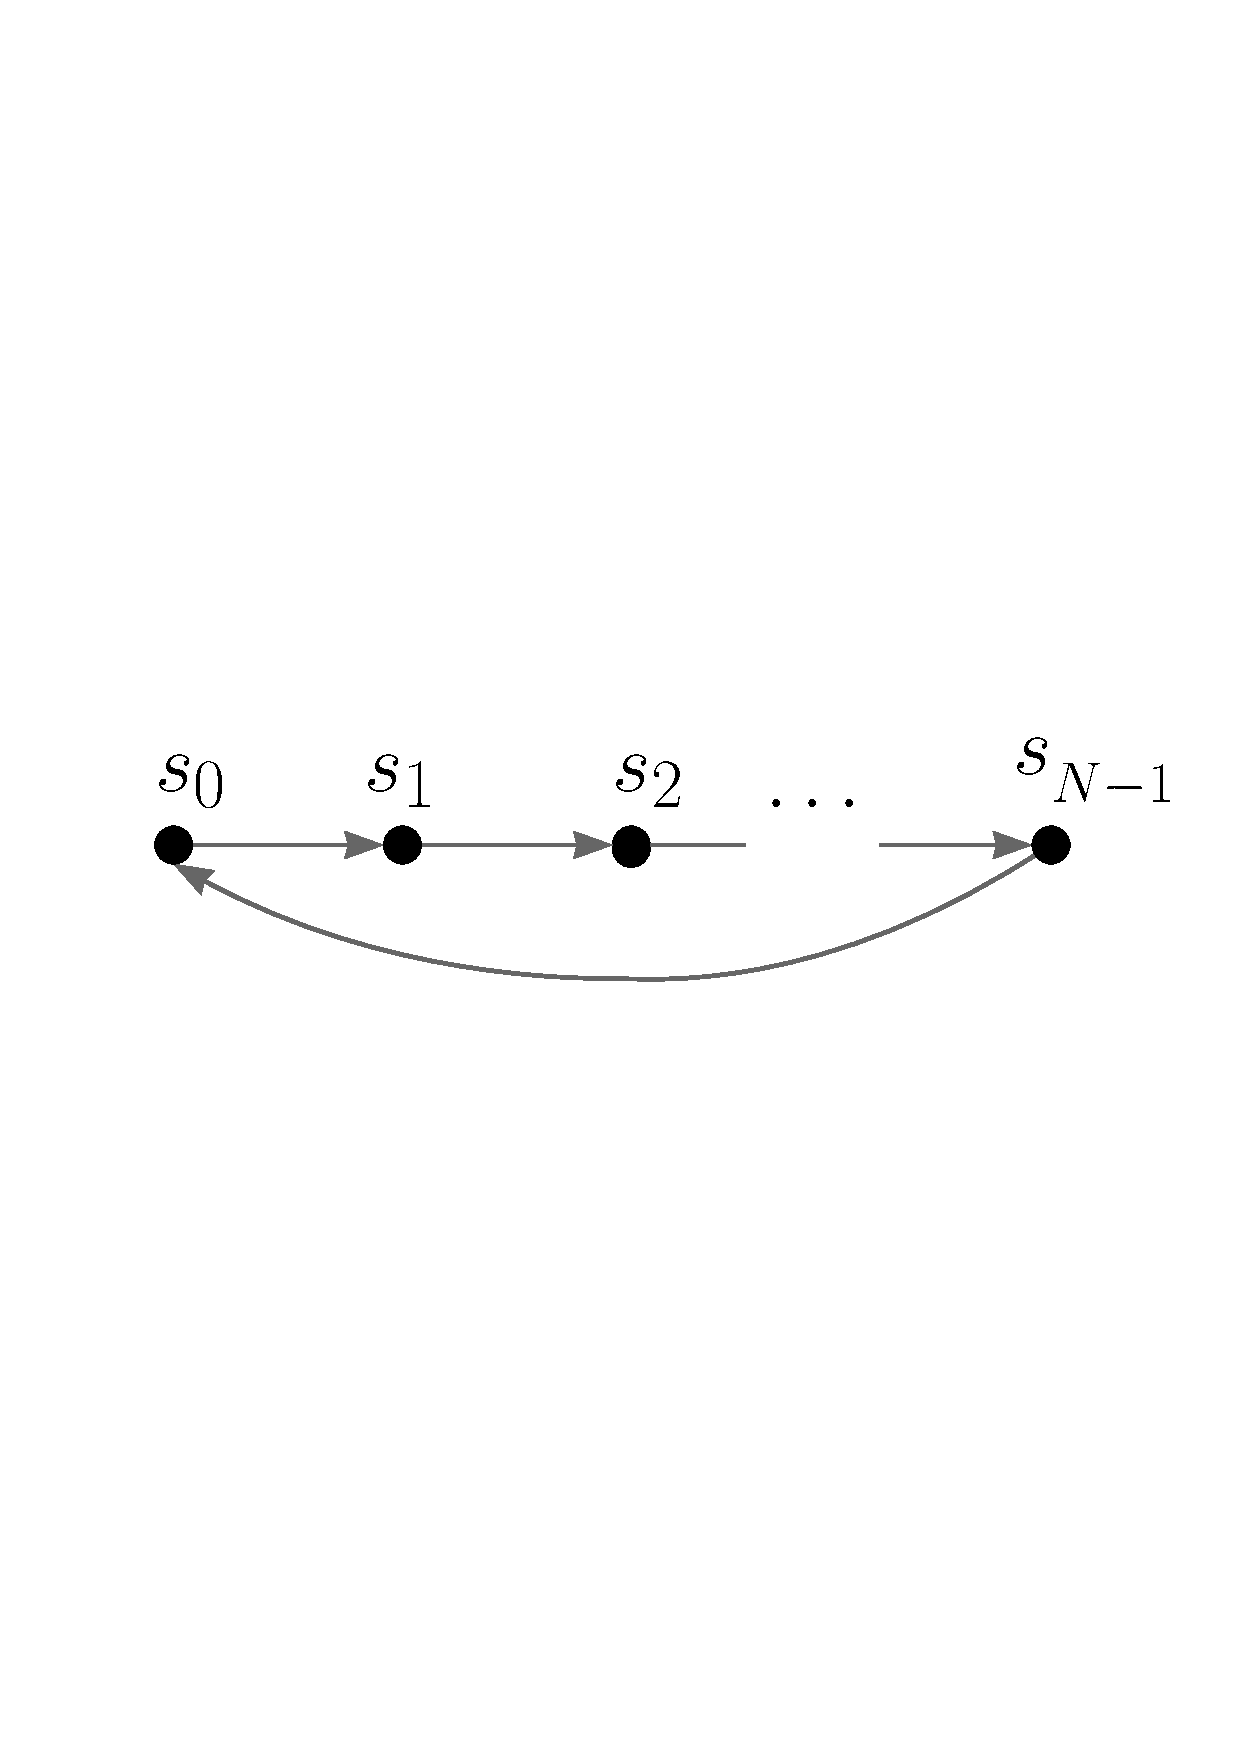
\includegraphics[width=0.45\linewidth]{Figures/signal_ring_graph_white_border.pdf} }}\hspace{0.2cm}%
% %	\qquad
% %	\subfloat[t][\label{figb_graphs}]{{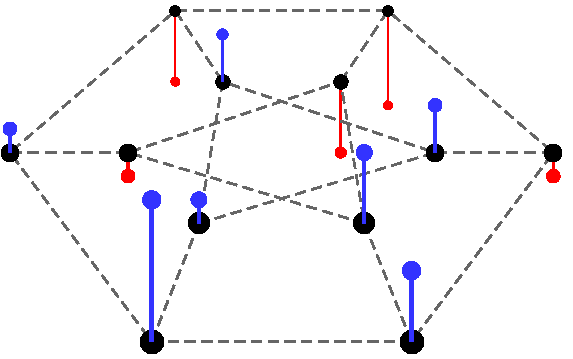
\includegraphics[width=0.4\linewidth]{Figures/signal_duher_graph.pdf} }}\\
% %	\subfloat[\label{figc_graphs}]{{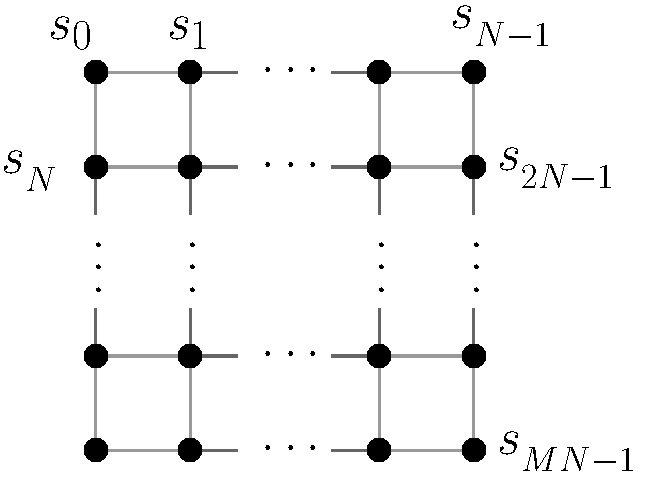
\includegraphics[width=0.45\linewidth]{Figures/image_graph.pdf} }}%
% %	\subfloat[\label{figd_graphs}]{{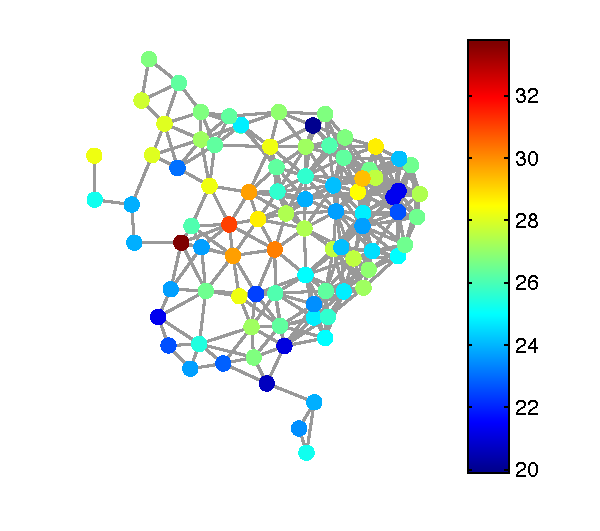
\includegraphics[width=0.4\linewidth]{Figures/graph_temp_bulbo_seco_NE_00h_01Fev2012_cropped.pdf} }}%
% %	\caption{Exemplos de representa\c{c}\~oes de sinais sobre (a) um grafo em anel direcionado, (b) um grafo de D\"{u}her n\~ao-direcionado, (c) um grafo n\~ao-direcionado em forma de rede retangular uniforme  e (d) um grafo formado por cidades do Nordeste brasileiro.}%
% %	\label{fig:graphs}%
% %	\vspace{-0.2cm}
% %\end{figure}
% \begin{equation}\label{eq:C}
% \mathbf{C} =
% \begin{bmatrix}
% &  &  &   1\\ 
% 1 &  &   & \\ 
% &   \ddots &  & \\ 
% &  &   1 & 
% \end{bmatrix},
% \end{equation}
% \noindent and plays an essential role in GSP: if a signal $ \mathbf{x} = (x_0 \ x_1 \ \dots \ x_{N-1})^T $ defined on a ring graph is left multiplied by the adjacency matix, one has $ \widetilde{\mathbf{x}} = (s_{N-1} \ x_0 \ \dots \ s_{N-2})^T $; that is,
% \begin{equation}\label{eq:graph_shift_C}
% \widetilde{\mathbf{x}} = \mathbf{C} \mathbf{x}
% \end{equation}
% \noindent is the result of circularly shifting $ \mathbf{x} $ to the right. This property suggests to generalize the unit shift of a signal on an arbitrary graph as being the left product by the corresponding adjacency matrix,
% \begin{equation}\label{eq:graph_shift_A}
% \widetilde{\mathbf{x}} = \mathbf{A} \mathbf{x},
% \end{equation}
% \noindent so that $ \mathbf{A} $ can be interpreted as the graph shift operator. In fact, this operator is a delay \emph{filter} for graph signals.

% A filter for signals on a graph with $ |\mathcal{V}| = N $ vertices can be defined as being any matrix $ \mathbf{H} \in \mathbb{C}^{N \times N} $ \cite{sandryhaila2013discrete}. Therefore, every graph filter is linear. On the other hand,
% \begin{equation}\label{eq:shift_invariance}
% \mathbf{HA}\mathbf{x} = \mathbf{AH}\mathbf{x},\:\:\forall \mathbf{x} \in \mathcal{S} \:\:\Leftrightarrow\:\:\mathbf{HA} = \mathbf{AH},
% \end{equation}
% \noindent that is, $ \mathbf{H} $ is a linear and shift-invariant (LSI) filter if and only if it commutes with the adjacency matrix $ \mathbf{A} $. The following theorem establishes an important property satisfied by every LSI filter~\cite{sandryhaila2013discrete} .
% \vspace{0.2cm}
% \begin{theorem}
% 	\label{theo:01}
% 	Let $ \mathbf{A} $ be the adjacency matrix of a graph. Let us assume that the characteristic polynomial $char_{\mathbf{A}}(x)$ of $\mathbf{A}$ coincides with the respective minimal polynomial $m_{\mathbf{A}}(x) $. Therefore, $ \mathbf{H} $ is a LSI filter if and only if $ \mathbf{H} $ is a polynomial in $ \mathbf{A} $, i.~e.
% 	\begin{equation}\label{eq:filtro}
% 	\mathbf{H} = h(\mathbf{A}) = \sum_{\ell=0}^{L} h_\ell \mathbf{A}^\ell,
% 	\end{equation}
% where $ \mathbf{A}^0 $ is the identity matrix and $ L < \deg(m_{\mathbf{A}}) $.
% \end{theorem}

% The assumption on $char_{\mathbf{A}}(x)$ and $m_{\mathbf{A}}(x)$ in Theorem~\ref{theo:01} does not hold for all adjacency matrices $\mathbf{A}$. Nevertheless, the result in the referred theorem can be extended to all matrices using the concept of \emph{equivalent graph filters}, as clearly explained in~\cite{sandryhaila2013filters}. In short, for any graph $\mathcal{G} = \{\mathbf{A}, \mathcal{V}\}$, every LSI filter has polynomial representation in $\mathbf{A}$. In this sense, Theorem~\ref{theo:01} suggests a convenient analogy with the classical DSP, since every filter for discrete-time signals can be represented as polynomials evaluated in $ z^{-1} $, the unit delay, via the $z$-transform of its impulse response.

% \begin{figure}[t!]
% 	\centering
% 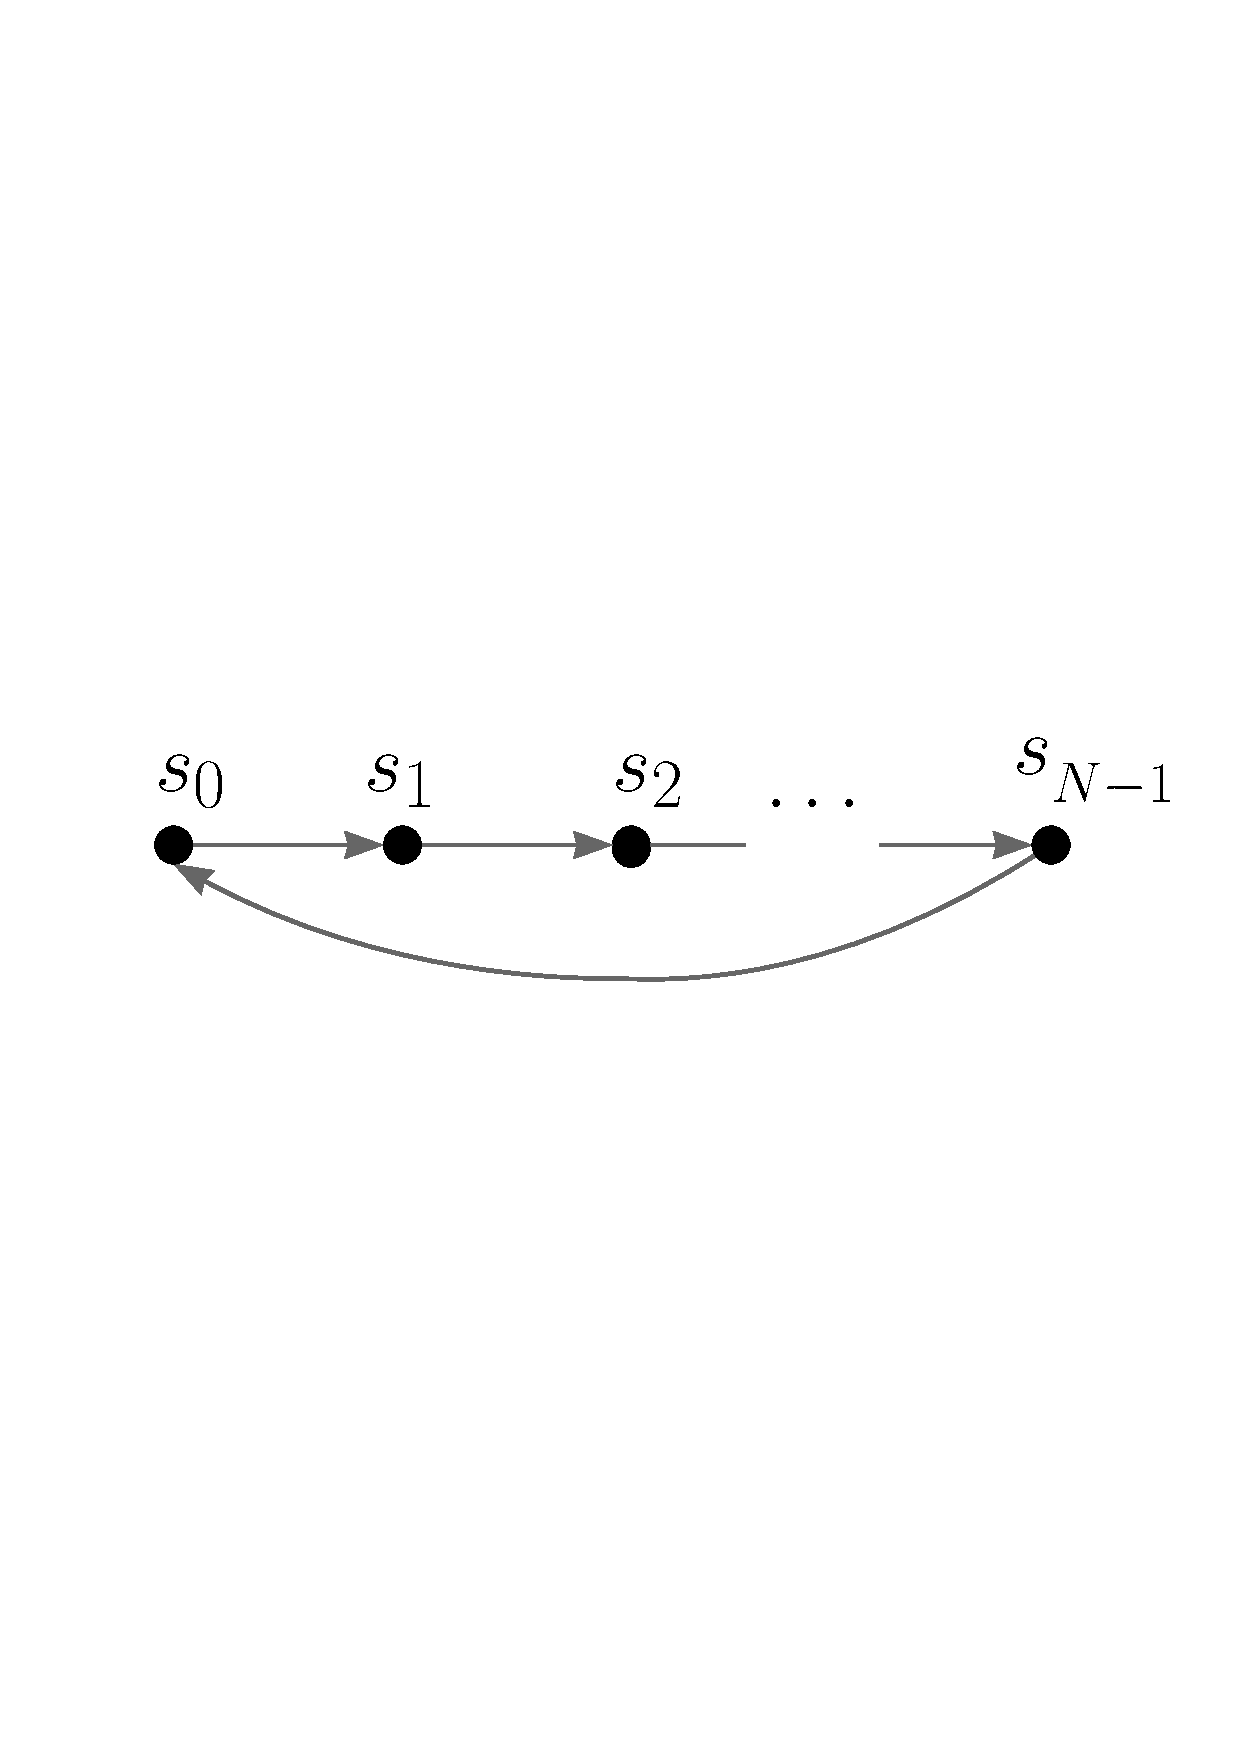
\includegraphics[width=0.3\linewidth]{Figures/signal_ring_graph_white_border.pdf}
% 	\caption{A directed ring graph.}%
% 	\label{fig:graphs}%
% 	\vspace{-0.5cm}
% \end{figure}
% \subsection{Graph Fourier Transform}

% The graph Fourier transform of a signal is its projection on a basis formed by functions invariant to linear and time-invariant (LTI) filtering~\cite{oppenheim1997signals}. Analogously, the graph Fourier transform (GFT) can be defined as the decomposition of a signal on a basis formed by eigenvectors of LSI filtering. Since LSI filters are polynomials in $ \mathbf{A} $ (Theorem \ref{theo:01}), and considering that a matrix and its integer powers share the same eigenvectors, the referred basis coincides with that obtained from the decomposition of $\mathbf{A}$~\cite{sandryhaila2013gft}. In this context, if the corresponding graph has $ N $ vertices, $\mathbf{A} $ admits the Jordan decomposition
% \begin{equation}\label{eq:gft_01}
% \mathbf{A} = \mathbf{V} \mathbf{J} \mathbf{V}^{-1},
% \end{equation}
% in which $ \mathbf{V} $ contains the $ N $ Jordan (generalized) eigenvectors of $ \mathbf{A} $ in its columns,
% \begin{equation}\label{eq:gft_02}
% \mathbf{V} = \left(\mathbf{v}_0 \ \mathbf{v}_1 \ \dots\ \mathbf{v}_{N-1}\right),
% \end{equation}
% and $\mathbf{J}$ is a block diagonal matrix formed of the so-called Jordan blocks. In particular, if $\mathbf{A}$ is diagonalizable, (\ref{eq:gft_01}) coincides with its eigendecomposition, so that $\mathbf{J}$ reduces to a diagonal matrix whose entries are the eigenvalues of $\mathbf{A}$.

% %Additionally, the subspaces generated by the eigenvectors of a given eigenvalue of $ \mathbf{A} $ are irreducible, have null intersection and have the sum of their dimensions totaling $ N $ \cite{sandryhaila2013gft}. Therefore, $ \mathbf{V} $ provides a basis invariant to LSI filtering for the signal space$ \mathcal{S} $ on the graph having $ \mathbf{A} $ as its adjacency matrix.

% In this manner, a signal $ \mathbf{x} \in \mathcal{S} $ can be decomposed into its components on the basis $ \mathbf{V} $ as
% \begin{align}\label{eq:GFT_inv}
% \mathbf{x} &= \widehat{x}_0 \mathbf{v}_0 + \dots + \widehat{x}_{N-1} \mathbf{v}_{N-1} \notag \\
% &= \mathbf{V} (\widehat{x}_0 \ \widehat{x}_1 \ \dots \ \widehat{x}_{N-1})^T \notag \\
% &= \mathbf{V} \widehat{\mathbf{x}}.
% \end{align}
% The last expression is then defined as being the synthesis equation of the graph Fourier transform. Consequently, the GFT analysis equation is
% \begin{equation}\label{eq:GFT_fwd}
% \widehat{\mathbf{x}} = \mathbf{V}^{-1} \mathbf{x}.
% \end{equation}

% For discrete-time signals, it has been remarked that the corresponding domain can be modeled as a directed ring graph with edges having unitary weights and, therefore, with adjacency matrix $ \mathbf{C} $ given in~(\ref{eq:C}). Since $ \mathbf{C} $ is circulant, it is diagonalized by the discrete Fourier transform (DFT) matrix $ \mathbf{F} $. Thus, one has
% \begin{equation}\label{eq:diag_C}
% \mathbf{C} = \mathbf{F}^{-1} \mathbf{\Lambda}_{\mathbf{C}} \mathbf{F},
% \end{equation}
% where $$ \mathbf{\Lambda}_{\mathbf{C}} = \text{diag}\left(
% 1 \:\
% e^{-j \frac{2\pi}{N}} \:\:\
% e^{-j \frac{4\pi}{N}}\:\: \
% e^{-j \frac{6\pi}{N}} \:\: \cdots \:\:
% e^{-j \frac{2\pi (N-1)}{N}}
% \right).$$In this case, the GFT matrix becomes $ \mathbf{V}^{-1} = \mathbf{F} $, evidencing the desirable property that the GFT of discrete-time signals coincides with the DFT.

% \vspace{0.25cm}
% \noindent\textbf{Frequency response of graph filters.} In order to understand how a graph filter acts on the GFT domain, identified as frequency domain,~(\ref{eq:gft_01}) and Theorem \ref{theo:01} are used. The response of the filter $ \mathbf{H} =\sum_{\ell=0}^{L} h_\ell \mathbf{A}^\ell $ to the signal $ \mathbf{x} $ is given by
% \begin{align}\label{eq:resposta_freq_01}
% \mathbf{H} \mathbf{x} &= \sum_{\ell=0}^{L} h_\ell \mathbf{A}^\ell \mathbf{x} =
% \sum_{\ell=0}^{L} h_\ell \left(\mathbf{V} \mathbf{J} \mathbf{V}^{-1}\right)^\ell \mathbf{x} \notag \\[0.5em]
% &= \mathbf{V} \left(\sum_{\ell=0}^{L} h_\ell \mathbf{J}^\ell \right) \mathbf{V}^{-1} \mathbf{x}.
% \end{align}
% Taking the GFT of both sides of the last equation, one has
% \begin{equation}\label{eq:resposta_freq_02}
% \mathbf{V}^{-1} \mathbf{H} \mathbf{x} =
% h(\mathbf{J}) \widehat{\mathbf{x}},
% \end{equation}
% so that the frequency domain equation corresponding to filtering using $ \mathbf{H} $ is the multiplication by the matrix $ h(\mathbf{J}) $, which represents the frequency response of the filter $ \mathbf{H} $.

\section{Fractional Shift on Graphs}\label{sec:fracshift}
Since the unit shift of a graph signal can be defined as the product by the adjacency matrix of the graph on which it lies, in this work, the proposed definition of a graph fractional shift as the product by a non-integer power of $ \mathbf{A} $. Precisely, the signal $\mathbf{x}$ over the graph $\mathcal{G} = \{ \mathbf{A}, {\mathcal{V}} \}$, after being shifted by $a\in[0,1]$, is given by
\begin{equation}
    \label{eq:def_frac_delay}
    \widetilde{\mathbf{x}}_a = \mathbf{A}^a \mathbf{x}.
\end{equation}
The following sections discuss aspects related to the computation of $\mathbf{A}^a$, the interpretation of its application to a graph signal and the consistency of the proposed operator with the classical DSP approach (ideal fractional delay filter).

\subsection{Computation of $\mathbf{A}^{{a}}$}\label{subsec:comp}
The computation of $\mathbf{A}^a$ can be well established by employing results from the theory of matrix functions~\cite{higham2008functions}. In this context, it suffices to evaluate the originally scalar function $f(t)=t^a$, $a\in\mathbb{R}$ having $\mathbf{A}$ as argument. The most direct way to formally define a function like this uses the Jordan canonical form. With this purpose, let us reconsider (\ref{eq:gft_01}), replacing the diagonalization of $\mathbf{A}$ with the most general decomposition
\begin{equation}
    \label{eq:Ajordan}
    \mathbf{A} = \mathbf{V} \mathbf{J} \mathbf{V}^{-1},
\end{equation}
using the Jordan block diagonal matrix $\mathbf{J}$,
\begin{equation}\label{eq:jcf}
    \mathbf{J}=\mathrm{diag}(\mathbf{J}_1,\mathbf{J}_2,\ldots,\mathbf{J}_p),
\end{equation}
and the matrix $\mathbf{V}$ of generalized eigenvectors. Each $k$-th Jordan block $\mathbf{J}_k$ is
\begin{equation}
    \mathbf{J}_k=\mathbf{J}_k(\lambda_k)=\left[\begin{array}{cccc}
            \lambda_k & 1         &        &           \\
                      & \lambda_k & \ddots &           \\
                      &           & \ddots & 1         \\
                      &           &        & \lambda_k
        \end{array}\right]\in\mathbb{C}^{m_k\times m_k}
\end{equation}
and $m_1+m_2+\ldots +m_p=N$. Denote by $\lambda_1,\ldots,\lambda_s$ the distinct eigenvalues of $\mathbf{A}$ and by $n_i$ the \emph{index} of $\lambda_i$ (the order of the largest Jordan block in which $\lambda_i$ appears). The function $f$ is said to be defined on the spectrum of $\mathbf{A}$ if the values
\begin{equation}\label{eq:defspec}
    f^{(j)}(\lambda_i),\quad j=0,1,\ldots,n_i-1,\quad i=1,2,\ldots,s,
\end{equation}
exist, where $f^{(j)}$ denotes the $j^{\textrm{th}}$ derivative of $f$.\footnote{As usual, the notation $f'$ will be used interchangeably with $f^{(1)}$.} That holds true for $f(t)=t^a$. The computation of $f(\mathbf{A})=\mathbf{A}^a$ can then be carried out as follows.
\vspace{0.2cm}
\begin{definition}\label{def:jc01}
    Let $f$ be defined on the spectrum of $\mathbf{A}\in\mathbb{C}^{N\times N}$ and let $\mathbf{A}$ have the Jordan decomposition~(\ref{eq:Ajordan}). Then
    \begin{equation}\label{eq:jcf01}
        f(\mathbf{A})\overset{\Delta}{=}\mathbf{V}f(\mathbf{J})\mathbf{V}^{-1}=\mathbf{V} \ \mathrm{diag}(f(\mathbf{J}_k)) \ \mathbf{V}^{-1},
    \end{equation}
    where
    \begin{equation}\label{eq:jcf02}
        f(\mathbf{J}_k)\overset{\Delta}{=}\left[\begin{array}{cccc}
                f(\lambda_k) & f'(\lambda_k) & \cdots & \frac{f^{(m_k-1)}(\lambda_k)}{(m_k-1)!} \\
                             & f(\lambda_k)  & \ddots & \vdots                                  \\
                             &               & \ddots & f'(\lambda_k)                           \\
                             &               &        & f(\lambda_k)\end{array}\right].
    \end{equation}
\end{definition}
In the present context, the last definition constitutes a practical way to calculate $\mathbf{A}^a$, because the Jordan form of the adjacency matrix, being necessary for the definition of the corresponding GFT, may already have been computed and thus be available to be used in~(\ref{eq:jcf01}) and~(\ref{eq:jcf02}).


\subsection{Interpreting the graph fractional shift}\label{subsec:interpret}
In order to perform a meaningful interpretation of the graph fractional shift, we consider~(\ref{eq:def_frac_delay}) and the case in which $\mathbf{A}$ is diagonalizable. Using the matrix factorization~(\ref{eq:gft_01}), the GFT analysis equation~(\ref{eq:GFT_fwd}) and the computation strategy described in the last subsection, we can write
\begin{align}\label{eq:frac_delay_01}
    \mathbf{A}^a \mathbf{x} & = \mathbf{V} \mathbf{\Lambda}^a \mathbf{V}^{-1} \mathbf{x} = \mathbf{V}
    \begin{bmatrix}
        \lambda_1^a &        &             \\
                    & \ddots &             \\
                    &        & \lambda_N^a
    \end{bmatrix}
    \widehat{\mathbf{x}} \notag                                                                                                                                         \\[0.5em]
                            & = \mathbf{V} (\widehat{\mathbf{h}}_a \odot \widehat{\mathbf{x}}) = \text{GFT}^{-1} \{\widehat{\mathbf{h}}_a \odot \widehat{\mathbf{x}}\},
\end{align}
where $\widehat{\mathbf{h}}_a \overset{\Delta}{=} (\lambda_1^a \ \ldots \ \lambda_N^a)^T$ and $\odot$ represents the point-wise vector product.

Equation~(\ref{eq:frac_delay_01}) shows that $ \mathbf{A}^a $ is a graph filter with frequency response $ \mathrm{diag}(\widehat{\mathbf{h}}_a) $; moreover, if $ \mathbf{x} $ is an $N$-point discrete-time signal (case in which the GFT coincides with the DFT), one observes that the filter in the DFT domain is the vector $ \widehat{\mathbf{h}}_a $ itself. In this case, it has been discussed that the adjacency matrix of the respective graph is diagonalized according with~(\ref{eq:diag_C}), where $ \mathbf{\Lambda}_{\mathbf{C}} $ has as entries the $ N $ roots of unity. The fact that the matrix of eigenvectors of $ \mathbf{C} $ is the Fourier matrix imposes a specific order of the eigenvalues in $ \mathbf{\Lambda}_{\mathbf{C}} $, so that the vector $ \widehat{\mathbf{h}}_a$ is
\begin{align*}
    \widehat{\mathbf{h}}_a & = (1 \,\, W_N^a \,\,W_N^{2a}\ldots W_N^{aR} \,\,W_N^{-aR'} \,\,W_N^{a(-R' + 1)}\ldots W_N^{-a}),
\end{align*}
where $ W_N = e^{-j \frac{2\pi}{N}} $ and
\begin{equation}
    \begin{cases}
        R = \frac{N-1}{2} \text{ and } R' = R,     & \text{ if } N \text{ is odd},\vspace{0.2cm} \\
        R = \frac{N}{2} - 1 \text{ and } R' = R+1, & \text{ if } N \text{ is even},
    \end{cases}
\end{equation}
$n=0,1,\ldots,N-1$. It can be shown that the inverse DFT of $ \widehat{\mathbf{h}}_a $ has components given by~(\ref{eq:DFT_inversa_autovalores}).

\begin{figure*}%[h!]
    \begin{equation}\label{eq:DFT_inversa_autovalores}
        h_a[n]\hspace{-0.03cm}=\hspace{-0.03cm}
        \left\{\begin{array}{ll}
            %\displaystyle
            {\dfrac{1}{N}} \dfrac{\sin (\pi (n-a))}{\sin \left(\frac{\pi}{N} (n-a)\right)},                             & \text{ if $N$ is odd},\vspace{0.25cm} \\
            %\displaystyle
            {\dfrac{1}{N} \cot \left(\dfrac{\pi}{N} (n-a)\right) \sin (\pi (n-a))}{+ \dfrac{j}{N} (-1)^n \sin (\pi a)}, & \text{ if } N \text{ is even}.
        \end{array}\right.
    \end{equation}
    % \hrule
\end{figure*}

\begin{figure}[b]
    \centering
    \subfloat[\label{figa_frac_delay_directed}]{{
                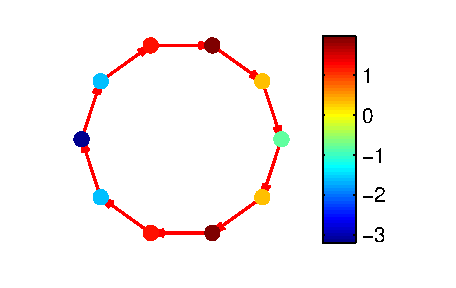
\includegraphics[width=0.35\linewidth]{Figures/d170309_frac_delay_ring_visualization_V5_a.eps}
            }}
    %	\vspace{-0.2cm}
    \subfloat[\label{figb_frac_delay_directed}]{{
                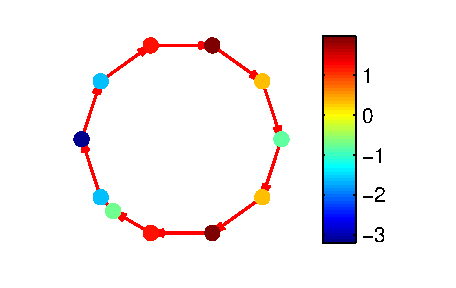
\includegraphics[width=0.35\linewidth]{Figures/d170309_frac_delay_ring_visualization_V5_b.eps}
            }}\\
    \subfloat[\label{figc_frac_delay_directed}]{{
                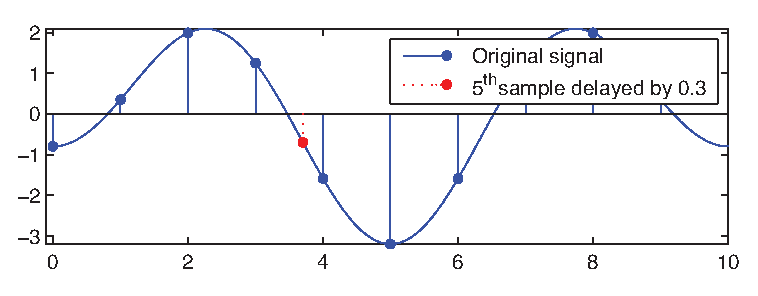
\includegraphics[width=0.6\linewidth]{Figures/d170309_frac_delay_ring_visualization_V5_c1.eps}
            }}% 
    \caption{Fractional shift by $a=0{.}3 $ of a sample of a signal on a directed ring graph with unit weights. (a) Original signal on a directed ring graph. (b) Graph in which the 5$\textsuperscript{th}$ sample delayed by $a=0{.}3 $ appears as an interpolated sample between the 4$\textsuperscript{th}$ and the 5$\textsuperscript{th}$ samples of the original signal. (c) Original discrete signal and the delayed sample.}
    \label{fig:frac_delay_directed}
    %\vspace{-0.3cm}
\end{figure}

The product by a fractional power of the adjacency matrix produces the effect illustrated in Fig. \ref{fig:frac_delay_directed}, for a directed ring graph; it can be seen, for example, how the 5\textsuperscript{th} sample of the signal shifted by $a=0{.}3 $ coincides with the value of the continuous-time signal at the same position. On the other hand, the analysis we can perform by observing the \textit{irregular} graph in Fig.~\ref{fig:sinal_Pernambuco} is mostly visual; as we vary the fractional parameter from $0$ (original signal) to $1$, we see in the intermediate snapshots how the signal gradually spreads out from the vertices where, originally, there were already non-zero samples. In this scope, although we employ terms such as delay and shift, which are inherited from classical signal processing, the process observed in the figure looks more like a kind of (fractional) diffusion. In fact, diffusion on graphs have been widely studied~\cite{zhang2008,thanou2017, benzi2021}; it is usually described in terms of a system of ordinary differential equations in time, with the Laplacian matrix of the graph as the coefficient matrix. Fractional diffusion has been used to model certain phenomena that allow long-range interactions and are non-local in nature~\cite{ilic2005,riascos2014,estrada2021,antil2021}.

Finally, it matters to highlight the fact that the signal to be shifted has to be bandlimited (see Fig.~\ref{figa_gibbs}). If the signal has abrupt changes in its sample values, this can be viewed as a kind of descontinuity and represents high frequency components, when compared to the predominantly smooth behavior of the signal (see Fig.~\ref{figb_gibbs}). As a consequence, we can observe considerable fluctuations around the disparate samples when the signal is fractionally delayed, an effect similar to the Gibbs phenomenon.

\begin{figure}[t!]
    \centering
    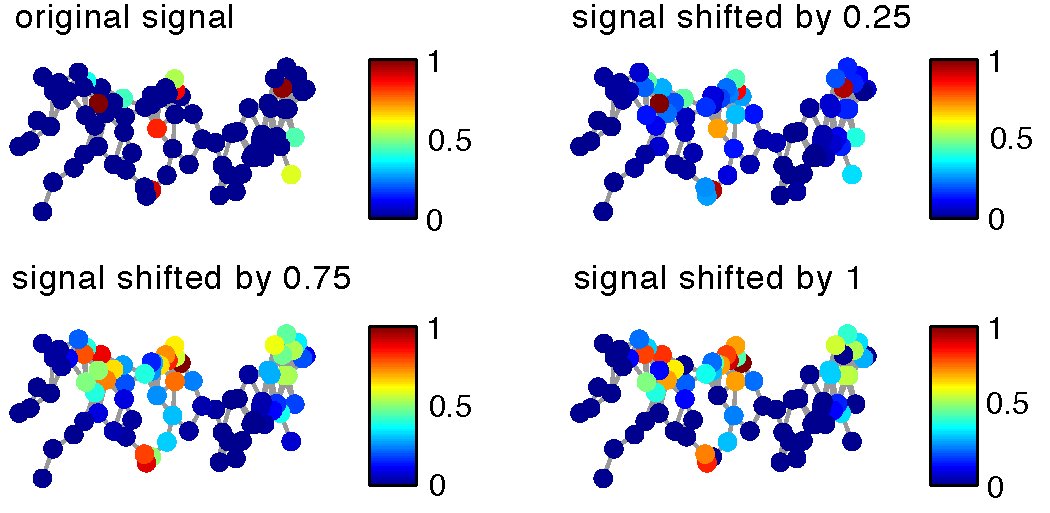
\includegraphics[width=0.6\linewidth]{Figures/signal_PE_V2_PT.pdf}
    \caption{Fractional shift of a signal, (originally) with $10$ non-zero samples, defined on a graph formed by $80$ cities of Pernambuco state, Brazil. Note that the shifted signal is similar to the original signal, if $ a $ is close to $0$, and similar to the unit-shifted signal, if $ a $ is close to $1$.}%
    \label{fig:sinal_Pernambuco}%
    \vspace{-0.2cm}
\end{figure}

\begin{figure}[t!]
    \centering
    \subfloat[\label{figa_gibbs}]{{
                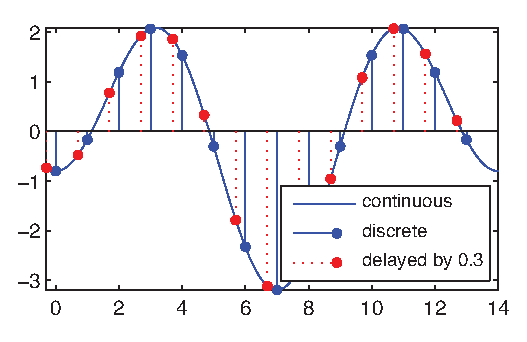
\includegraphics[width=0.4\linewidth]{Figures/d170309_frac_delay_ring_visualization_V2_no_gibbs.eps}
            }}~
    %	\vspace{-0.2cm}
    \subfloat[\label{figb_gibbs}]{{
                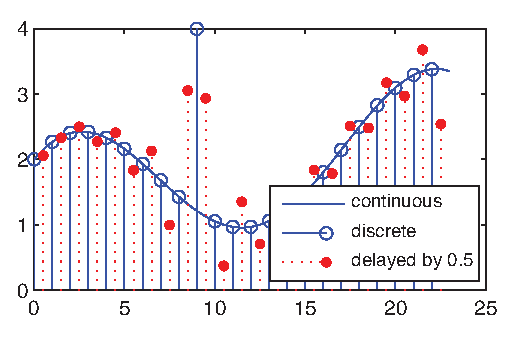
\includegraphics[width=0.4\linewidth]{Figures/frac_delay_ring_TESTS_gibbs_effect.eps}
            }}%
    \caption{Fractional shift for a signal (a) without and (b) with abrupt variations (descontinuities).}%
    \label{fig:frac_delay_gibbs}%
    \vspace{-0.2cm}
\end{figure}

\subsection{Consistency with classical approach: the ideal fractional delay filter}\label{subsec:consist}
In the classical approach to the problem of fractionally shifting a discrete-time signal, the continuous-time version of the signal can be reconstructed, shifted and then resampled with the same sampling period~\cite{alan1989discrete,valimaki1995discrete}. Due to the Nyquist-Shannon Theorem, this procedure requires that the signal is bandlimited. In this context, it can be shown that, if a discrete-time signal $ \mathbf{x} $ is bandlimited, its version shifted by $ a \in [0,1] $ is
$$
    x[n-a] = \sum_k x[k] \mathrm{sinc} (n - k - a),
$$
so that the (ideal low-pass) filter used to perform the referred shift has components
\begin{equation}
    h_{_{LPF}}[n] = \mathrm{sinc} (n-a).
\end{equation}

The filter $ \mathbf{h}_{_{LPF}} $ is non-causal and unstable (it is not BIBO -- \emph{bounded input, bounded output}, because its impulse response has infinite energy) and, therefore, it is not physically realizable. In this way, fractional delay filter implementations should just \emph{approximate} $ \mathbf{h}_{_{LPF}} $ as much as possible.

In order to evaluate how close to $ h_{_{LPF}}[n] = \mathrm{sinc} (n-a) $, $ 0\leq a \leq 1 $, is $h_a[n]$, for odd $N$ (see the first row of~(\ref{eq:DFT_inversa_autovalores})), the point-wise difference between these signals has been computed for different values of $ N \in [10^1, 10^6]$. Fig. \ref{fig:convergence}, shows the relative error (ratio between the energy of the error $(\mathbf{h}_a - \mathbf{h}_{_{LPF}})$ and that of $ \mathbf{h}_{_{LPF}} $), in terms of $ N $ and $a $.

The result suggests that, in fact, $ \mathbf{h}_a $ converges in the mean in $ \ell^2 $ to $ \mathbf{h}_{_{LPF}}$ as $ N $ grows, with relative error less than $ 5\% $ for $ N \approx 30 $. Moreover, the error is greater when $ a $ is close to $ 0{.}5 $, being negligible or null when $ a $ is an integer. In fact, the error is exactly zero for $ a=0$ (or $a=1$) and $ n = a $, since
\begin{equation}\label{eq:lim_h_impar}
    \lim_{n \rightarrow a} h_{a}[n] = 1
    \Rightarrow
    \lim_{n \rightarrow a} \big(h_{a}[n] - \mathrm{sinc}(n-a)\big) = 0.
\end{equation}

The same result is obtained for even $N$, starting from the second row of~(\ref{eq:DFT_inversa_autovalores}). When $a$ is non-integer, $h_a[n] $ is complex, with imaginary part of constant modulus for a fixed $a$. Considering the corresponding real part only, the error was smaller than that taking into account also the contribution of the imaginary part. Fig. \ref{fig:convergence_even_N_real_part} and Fig. \ref{fig:convergence_even_N_abs} show that the errors with and without the imaginary part equally decay as  $ N $ grows, but, using the real part only, the results are significantly better.

\begin{figure}[ht!]
    \centering
    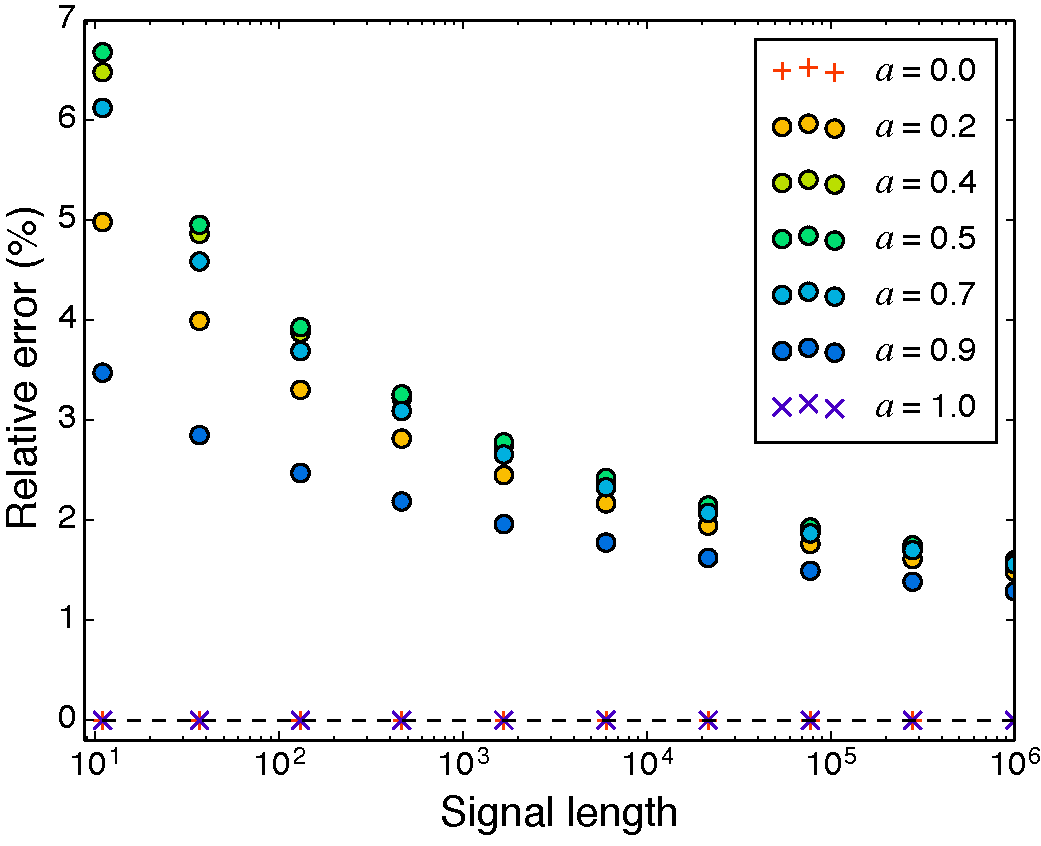
\includegraphics[width=0.5\linewidth]{Figures/convergence_odd_N_V4.pdf}
    \caption{Percent error (normalized by the energy of $ \mathbf{h}_{_{LPF}} $) of $ \mathbf{h}_a $ related to $ \mathbf{h}_{_{LPF}} $, for different (odd) values of $ N $ and the fractional shift parameter $ a $.}
    \label{fig:convergence}
\end{figure}

\begin{figure}[ht!]
    \centering
    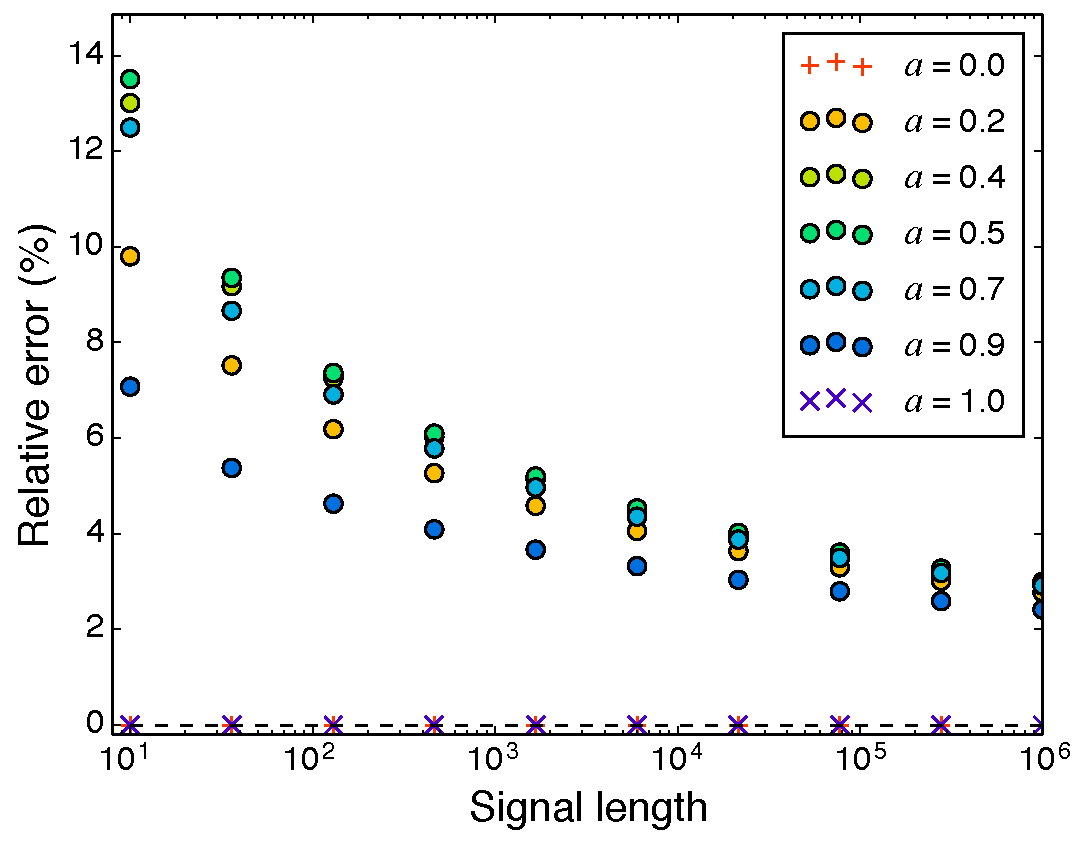
\includegraphics[width=0.5\linewidth]{Figures/convergence_even_N_real_part.pdf}
    \caption{Relative mean error between $ \mathcal{R}e\{\mathbf{h}_a\} $ and $ \mathbf{h}_{_{LPF}} $ for $ N $ even, in terms of the fractional shift parameter $a$.}
    \label{fig:convergence_even_N_real_part}
\end{figure}

\begin{figure}[ht!]
    \centering
    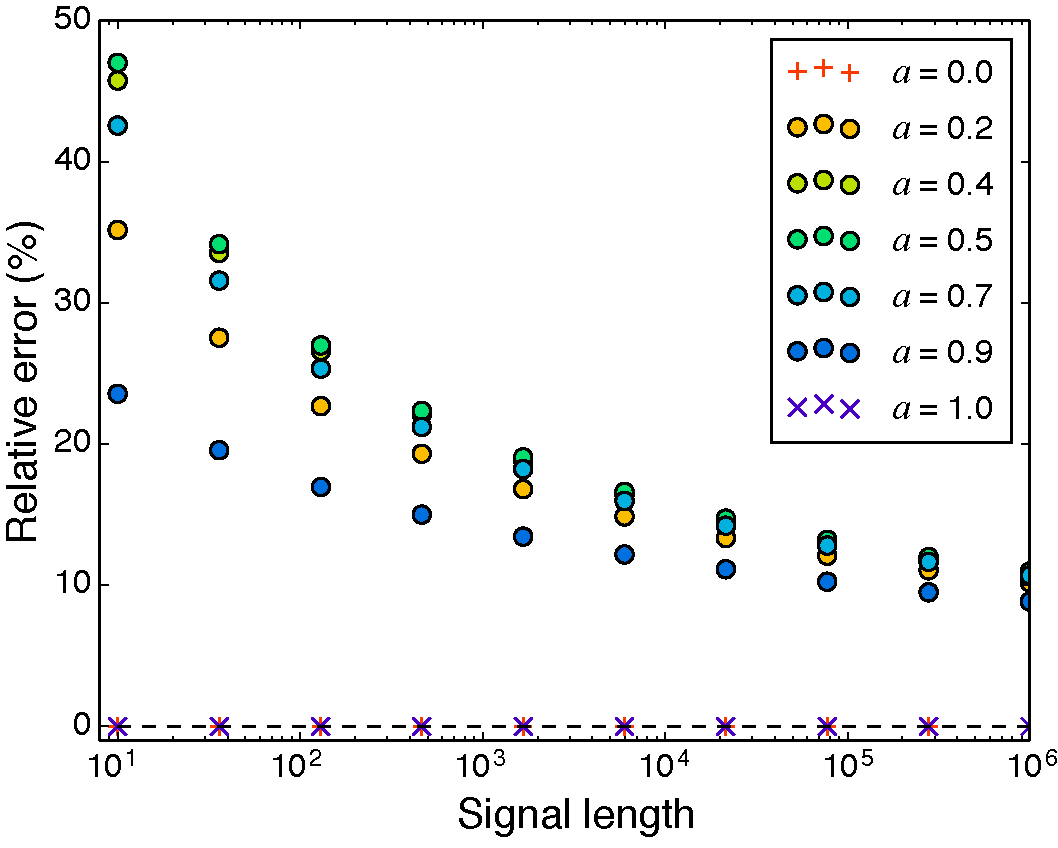
\includegraphics[width=0.5\linewidth]{Figures/convergence_even_N_abs_V2.pdf}
    \caption{Modulus of the relative mean error between $ \mathbf{h}_a $ and $ \mathbf{h}_{_{LPF}} $ for $ N $ even, in terms of the fractional shift parameter $a$.}
    \label{fig:convergence_even_N_abs}
    \vspace{-0.3cm}
\end{figure}

\subsection{Polynomial representation}\label{subsec:poly}
The fractional shift matrix $ \mathbf{A}^a$ necessarily commutes with $ \mathbf{A} $, because $ \mathbf{A}^a\mathbf{A} = \mathbf{A}^{1 + a} = \mathbf{A}\mathbf{A}^a  $, so that $ \mathbf{A}^a $ is an LSI filter for signals on graphs having  $ \mathbf{A} $ as adjacency matrix (see~(\ref{eq:lsi_def})). Therefore, according to Theorem~\ref{theo:01}, $\mathbf{A}^a$ admits a polynomial representation like the one given in~(\ref{eq:filtro}). In what follows, we evaluate such a possibility for directed ring graphs and for arbitrary graphs.

\vspace{0.25cm}
\noindent\textbf{Directed ring graphs.} The adjacency matrix $ \mathbf{C} $ in~(\ref{eq:C}) of the directed ring graph with unitary weights satisfies $ char_\mathbf{C} = m_\mathbf{C} $ (due to the fact that the eigenvalues of  $\mathbf{C}$ are distinct). Therefore $ \mathbf{H} = \mathbf{C}^a $ can be directly expressed as a polynomial of degree up to  $(N-1)$ in $ \mathbf{C} $. In order to do this, we consider ~(\ref{eq:diag_C}) and the fact that $ \mathbf{F}^{-1} = \mathbf{F}^H $, with $ H $ indicating the conjugate transpose. This allows to show that  $ \mathbf{C}^a = \mathbf{F}^{H} \mathbf{\Lambda}^a_{\mathbf{C}} \mathbf{F}$ is a circulant matrix with the first column given by $ \mathbf{h}_a $ in (\ref{eq:DFT_inversa_autovalores}). Moreover, since the left product of a matrix by $\mathbf{C}$ produces a circular down-shift in each column of the matrix, the $ N $ powers of $\mathbf{C}$ form a basis for the space of $N\times N $ circulant matrices (note that $\mathbf{C}^N =  \mathbf{C}^0$ is the identity matrix). From the above, we conclude that the coefficients of the polynomial representation of $ \mathbf{C}^a $ are the entries of $ \mathbf{h}_a $, i.~e.
\begin{equation}\label{eq:poly_C}
    \mathbf{H} = \mathbf{C}^a = \sum_{\ell=0}^{N-1} h_a[\ell] \mathbf{C}^\ell.
\end{equation}

\noindent\textbf{Arbitrary graphs.} In order to demonstrate how to obtain the polynomial representation of $\mathbf{H}=\mathbf{A}^a$ for arbitrary graphs, let us consider another strategy to compute matrix functions. By definition, the minimal polynomial $m_{\mathbf{A}}(t)$ of $\mathbf{A}$ is the unique monic polynomial of lowest degree such that $m_{\mathbf{A}}(\mathbf{A})=\mathbf{0}$. By considering the Jordan canonical form of $\mathbf{A}$, it can be seen that
\begin{equation}
    m_{\mathbf{A}}(t)=\prod_{i=1}^s (t-\lambda_i)^{n_i}.
\end{equation}
It follows immediately that $m_{\mathbf{A}}$ is zero on the spectrum of $\mathbf{A}$, that is, the values computed in~(\ref{eq:defspec}) are all zero for $f(t)=m_{\mathbf{A}}(t)$. Given any polynomial $p$ and any matrix $\mathbf{A}\in\mathbb{C}^{N\times N}$, $p$ is clearly defined on the spectrum of $\mathbf{A}$ and $p(\mathbf{A})$ can be defined by substitution. For polynomials $p$ and $q$, $p(\mathbf{A})=q(\mathbf{A})$ if and only if $p$ and $q$ take the same values on the spectrum. Thus the matrix $p(\mathbf{A})$ is completely determined by the values of $p$ on the spectrum of $\mathbf{A}$. The following definition can then be established.
\vspace{0.2cm}
\begin{definition}\label{def:jc02}
    Let $f$ be defined on the spectrum of $\mathbf{A}\in\mathbb{C}^{N\times N}$. Then $f(\mathbf{A})\overset{\Delta}{=}p(\mathbf{A})$, where $p$ is the unique polynomial of degree less than $\sum_{i=1}^s n_i$ (which is the degree of the minimal polynomial) that satisfies the interpolation conditions
    \begin{equation}
        p^{(j)}(\lambda_i)=f^{(j)}(\lambda_i),\quad j=0:n_i-1,\quad i=1:s.
    \end{equation}
\end{definition}

The polynomial $p$ above is known as the Hermite interpolating polynomial. In particular, if $n_i=1$, $i=1,\ldots,s$, $p$ corresponds to the Lagrange interpolating polynomial
\begin{equation}
    p(t)=\sum_{i=1}^s f(\lambda_i)l_i(t),\quad l_i(t)=\prod_{j=1,j\neq i}^s \left(\frac{t-\lambda_j}{\lambda_i-\lambda_j}\right).
\end{equation}
In any case, the results briefly presented above lead us to conclude that $\mathbf{A}^a$ can be expressed as a polynomial in $\mathbf{A}$ and, therefore, according to Theorem~\ref{theo:01}, the fractional shift of a graph signal can be implemented as an LSI graph filter.

\section{Numerical Results}\label{sec:num}
The last section discussed the effect of applying a fractional shift to a graph signal and demonstrated that $\mathbf{A}^a$ admits a polynomial representation. In the first part of this section, a brief numerical example is presented to illustrate how the referred representation can be obtained. Then, the proposed fractional operator is applied in a context which brings to the front its practical advantage, namely the design of graph filters. Naturally, the resulting filter, being a polynomial in $\mathbf{A}^a$, could also be expressed as a polynomial in $\mathbf{A}$ and, therefore, it is a LSI filter.

\subsection{Example: Polynomial Representation of $\mathbf{A}^{a}$}\label{subsec:num1}
The graph considered in this example is shown in Fig.~\ref{fig:polyrepres} and has adjacency matrix
\begin{equation}\label{eq:ex001}
    %\setlength{\arraycolsep}{3pt}
    \mathbf{A}=\left[\begin{array}{ccccc}
            5  & 4  & 2  & 1  \\
            0  & 1  & -1 & -1 \\
            -1 & -1 & 3  & 0  \\
            1  & 1  & -1 & 2
        \end{array}\right].
\end{equation}
The entries of $\mathbf{A}$ in~(\ref{eq:ex001}) were chosen so that the Jordan decomposition of such a matrix had integer entries only. The referred decomposition is written using matrices
\begin{equation}\nonumber
    %\setlength{\arraycolsep}{3pt}
    \mathbf{V}=\left[\begin{array}{ccccc}
            -1 & 1  & 1  & 1 \\
            1  & -1 & 0  & 0 \\
            0  & 9  & -1 & 0 \\
            0  & 1  & 1  & 0
        \end{array}\right],\:\:
    %\setlength{\arraycolsep}{3pt}
    \mathbf{V}^{-1}=\left[\begin{array}{ccccc}
            0 & 1 & 1  & 1 \\
            0 & 0 & 1  & 1 \\
            0 & 0 & -1 & 0 \\
            1 & 1 & 1  & 0
        \end{array}\right]
\end{equation}
and
\begin{equation}
    %\setlength{\arraycolsep}{3pt}
    \mathbf{J}=\left[\begin{array}{ccccc}
            1 & 0 & 0 & 0 \\
            0 & 2 & 0 & 0 \\
            0 & 0 & 4 & 1 \\
            0 & 0 & 0 & 4
        \end{array}\right].
\end{equation}
Considering $f(t)=t^{0.3}$ and Definition~\ref{def:jc01}, $f(\mathbf{A})=\mathbf{A}^{0.3}$ can be computed according to
\begin{equation}\nonumber
    %\setlength{\arraycolsep}{2.5pt}
    \mathbf{A}^{0.3}=\mathbf{V}
    \left[\begin{array}{ccccc}
            f(1) & 0    & 0    & 0     \\
            0    & f(2) & 0    & 0     \\
            0    & 0    & f(4) & f'(4) \\
            0    & 0    & 0    & f(4)
        \end{array}\right]\mathbf{V}^{-1},
\end{equation}
which gives
\begin{equation}\nonumber
    %\setlength{\arraycolsep}{2.5pt}
    \mathbf{A}^{0.3}=
    \left[\begin{array}{ccccc}
            1.6294  & 0.6294  & 0.3448  & 0.2311  \\
            0       & 1.0000  & -0.2311 & -0.2311 \\
            -0.1137 & -0.1137 & 1.4020  & 0       \\
            0.1137  & 0.1137  & -0.1709 & 1.2311
        \end{array}\right].
\end{equation}
The same result can be achieved by using Definition~\ref{def:jc02}, which gives
\begin{align}
    p(\mathbf{A}) & =f(\mathbf{A})=\mathbf{A}^{0.3}\nonumber                                           \\
                  & =0.6688\mathbf{I}+0.3915\mathbf{A}-0.0654\mathbf{A}^2+0.0051\mathbf{A}^3,\nonumber
\end{align}
the polynomial representation of $\mathbf{A}^{0.3}$.

\begin{figure}
    \centering
    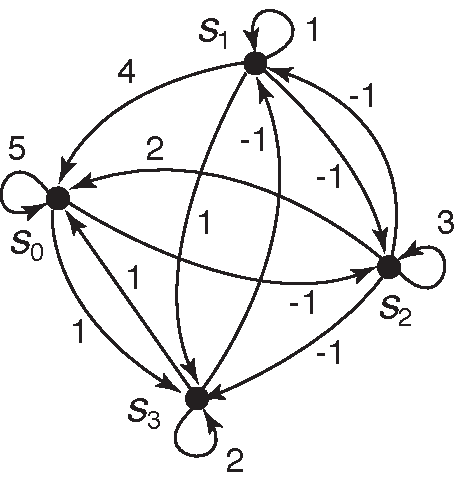
\includegraphics[width=0.35\linewidth]{Figures/graph_jordan.pdf}
    \caption{Directed graph used to illustrate how the corresponding fractional shift operator can be computed and represented in polynomial form.}
    \label{fig:polyrepres}
\end{figure}

\subsection{Least-square approximation of LSI filters}\label{subsec:lsi}
Before developing a numerical example illustrating the use of $\mathbf{A}^a$ to filter graph signals, let us first review a simple design technique that are least-squares approximations of ideal LSI filters~\cite{sandryhaila2014frequency}. Such a method consists of defining the (ideal) filter by specifying the values of $h(\lambda_i)$ (filter response in each eigenvalue of the shift operator), instead of determining the values of $h_{\ell}$ (filter coefficients). Describing the frequency response of the filter for each eigenvalue  $ \lambda_i $ yields the linear system of equations
\begin{equation}
    \label{eq:siseq}
    \begin{aligned}
        h(\lambda_0)     & = \alpha_0,     \\
        h(\lambda_1)     & = \alpha_1,     \\
                         & \vdots          \\
        h(\lambda_{N-1}) & = \alpha_{N-1}, \\
    \end{aligned}
\end{equation}
or, since $ h(\cdot) $ is a polynomial of degree $ L $,
\begin{equation}\label{eq:syst01}
    \begin{aligned}
        h_0 + h_1 \lambda_0 + \dots + h_L \lambda^L_0         & = \alpha_0,     \\
        h_0 + h_1 \lambda_1 + \dots  + h_L \lambda^L_1        & = \alpha_1,     \\
                                                              & \vdots          \\
        h_0 + h_1 \lambda_{N-1} + \dots + h_L \lambda^L_{N-1} & = \alpha_{N-1}. \\
    \end{aligned}
\end{equation}
Using a Vandermonde matrix constructed from the eigenvalues $\lambda_i$, the system~(\ref{eq:syst01}) can be written in matrix form as
\begin{equation}\label{eq:siseq2}
    \setlength{\arraycolsep}{3pt}
    \left[\begin{array}{ccccc}
            1 & \lambda_0     & \lambda^2_0     & \dots  & \lambda^L_0     \\
            1 & \lambda_1     & \lambda^2_1     & \dots  & \lambda^L_1     \\
              & \vdots        &                 & \vdots &                 \\
            1 & \lambda_{N-1} & \lambda^2_{N-1} & \dots  & \lambda^L_{N-1} \\
        \end{array}\right]
    \begin{bmatrix}
        h_0    \\
        h_1    \\
        \vdots \\
        h_L
    \end{bmatrix} =
    \begin{bmatrix}
        \alpha_0 \\
        \alpha_1 \\
        \vdots   \\
        \alpha_{N-1}
    \end{bmatrix}.
\end{equation}
More specifically, if one desires to design a low-pass filter (LPF) whose cutoff frequency is $ \lambda_{i_\text{cut}} $, one could set
\begin{equation}
    \label{eq:alfas}
    \alpha_j =
    \left\{\begin{array}{ll}
        1, & \text{for } j = 0,\ldots, i_\text{cut},    \\
        0, & \text{for } j = i_\text{cut}+1,\ldots,N-1.
    \end{array}\right.
\end{equation}
Since one generally has $ N \geq L+1$, the system of equations~(\ref{eq:siseq2}) is \emph{overdetermined} and does not have an exact solution. A possible strategy is to find coefficients $ h_\ell $, $ \ell=0, \dots, L$, that minimize, in the least-squares sense, the deviation from the ideal filter response. This corresponds to solve the optimization problem
\begin{equation}
    \label{eq:opt}
    \underset{\{h_\ell\}_{0, \dots, L}}{\text{min}} \sum_{n=0}^{N-1} \left( h(\lambda_n) - \alpha_n \right)^2.
\end{equation}

\noindent\textbf{Proposed application of the fractional shift.} The proposed change to the method above, which includes the fractional shift in the filter design, consists of replacing $\mathbf{A}$ with $\mathbf{A}^a$ in~(\ref{eq:filtro}), representing the LSI filter as
\begin{equation}
    \label{eq:filtrofracnew}
    h(\mathbf{A}^a) = \sum_{\ell=0}^{L} h_\ell \mathbf{A}^{a \cdot \ell}.
\end{equation}
If this is performed, the only adjustment needed in the technique described above consists of replacing the eigenvalues $\lambda_i$ with their $a^{\text{th}}$ powers $\lambda_i^a$ in~(\ref{eq:syst01}). The effect of such a substitution is illustrated and evaluated in what follows.

\subsection{Example: LS Approximation using $\mathbf{A}^{{a}}$}\label{subsec:lsi01}
In this example, we consider a network formed by $230$ weather stations that measure daily temperature across the United States~\cite{data2011}. Such stations are represented by the vertices of an undirected graph whose edges have been established by using the $8$-nearest neighbor criterion.  The edge connecting vertices $v_n$ and $v_m$ is weighted according to
\begin{equation}
    \mathbf{A}_{n,m}=\frac{e^{-d^2_{n,m}}}{\sqrt{\sum_{k\in\mathcal{N}_n}e^{-d^2_{n,k}}\sum_{\ell\in\mathcal{N}_m}e^{-d^2_{n,\ell}}}},
\end{equation}
where $d_{n,m}$ denotes the geodesical distance between the $n^{\text{th}}$ and the $m^{\text{th}}$ sensors. The snapshot of all measurements taken on February $1^{\text{st}}$, 2003 forms the signal indexed by the referred graph, which is shown in Fig.~\ref{fig:usa00}. From the GFT of the signal, which is plotted in Fig.~\ref{fig:usa01}, it can be seen that its spectral content is concentrated in the low graph frequencies. Note that such frequencies correspond to the eigenvalues of $\mathbf{A}$, which are marked along the horizontal axis of the figure; additionally, the referred marking accompanies the fact that low (resp. high) graph frequencies are associated with higher (resp. lower) eigenvalues~\cite{sandryhaila2014frequency}.

\begin{figure}%
    \centering
    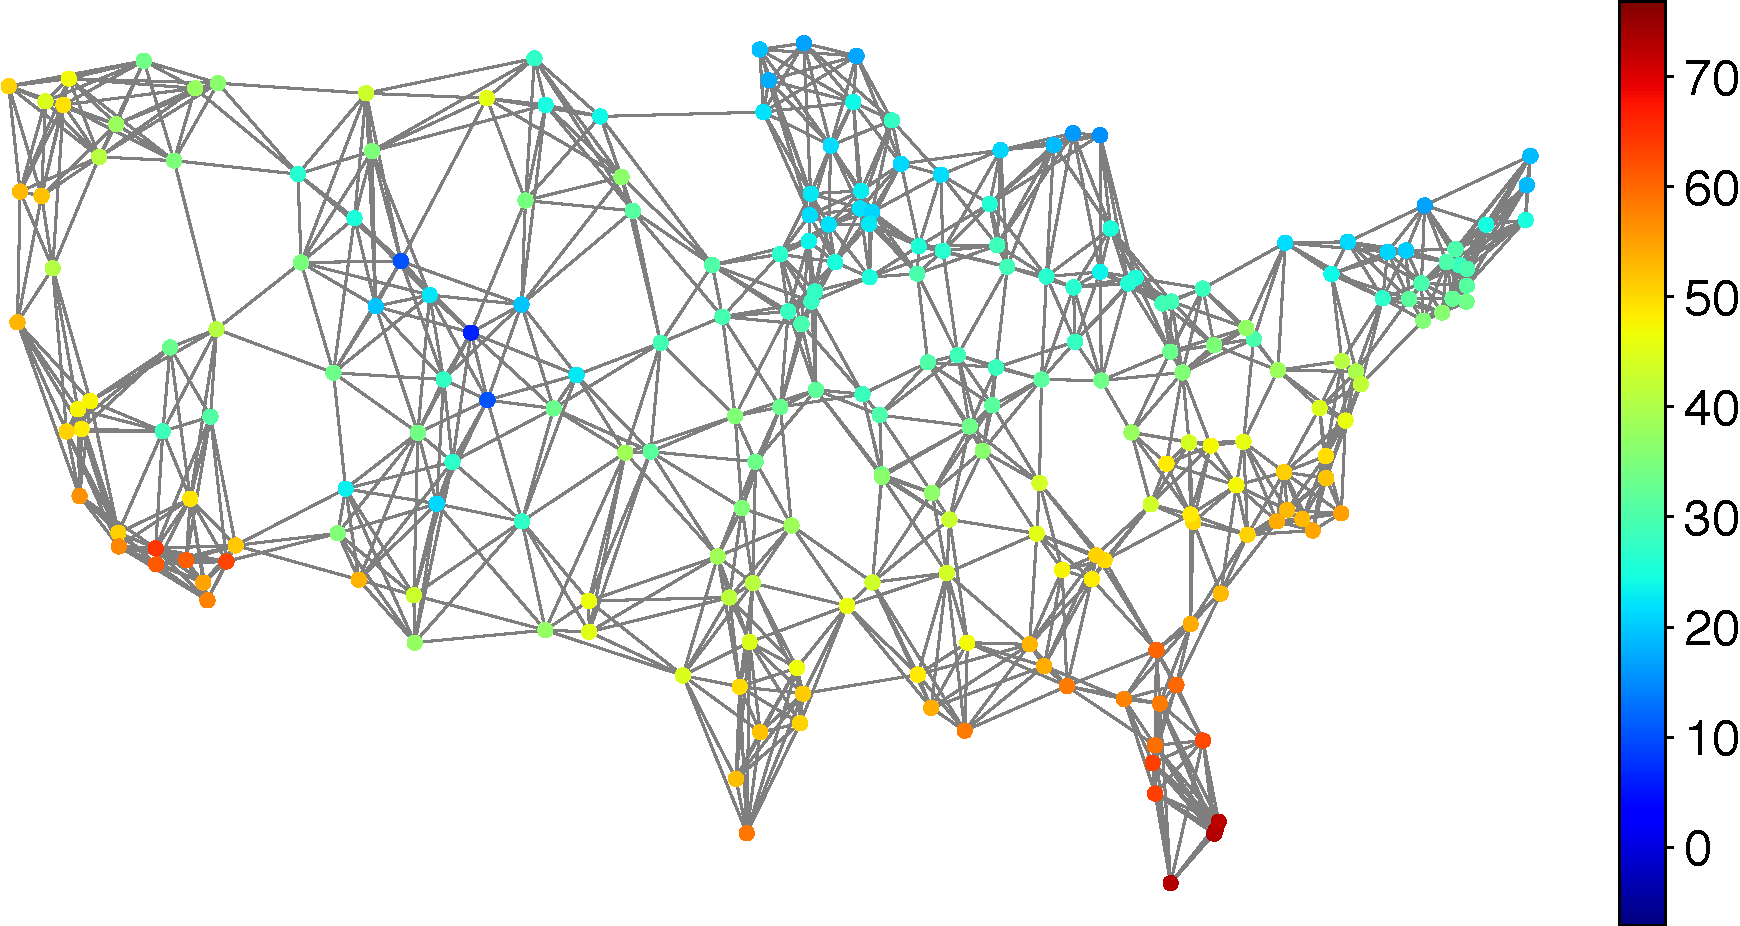
\includegraphics[width=0.6\linewidth]{Figures/GNorm_estacoes_temperatura.pdf}
    \caption{Graph of a network formed by $230$ weather stations measuring the temperature across the United States. The snapshot of all measurements taken on February $1^{\text{st}}$, 2003 is the corresponding graph signal.}%
    \label{fig:usa00}%
    \vspace{0.14cm}
\end{figure}

\begin{figure}[ht!]%
    \centering
    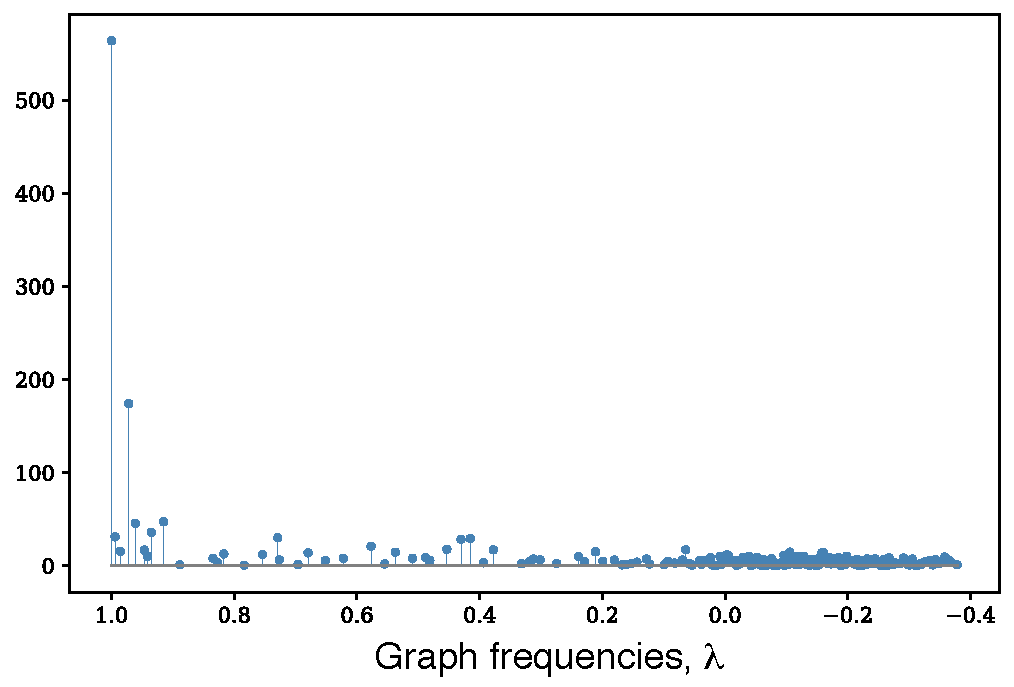
\includegraphics[width=0.5\linewidth]{Figures/GNorm_estacoes_GFT_Temperatura.pdf}%\vspace{-0.1cm}
    \caption{Magnitude of the graph Fourier transform of the signal in Fig~\ref{fig:usa00}. The graph frequencies correspond to the eigenvalues of $\mathbf{A}$; low (resp. high) graph frequencies are associated with higher (resp. lower) eigenvalues.}%
    \label{fig:usa01}%
    %\vspace{-0.2cm}
\end{figure}

\begin{figure}[ht!]
    \centering
    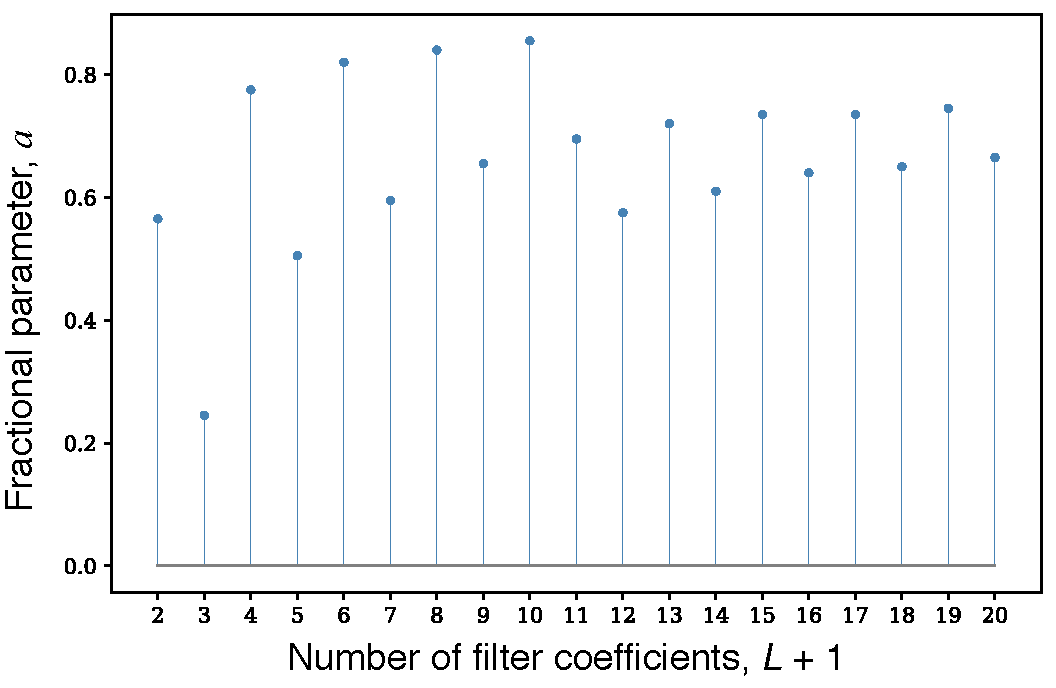
\includegraphics[width=0.5\linewidth]{Figures/ERROR_ordens_fracionarias.pdf}
    \caption{Fractional parameters providing the minimum approximation errors, for different values of $L$, between the ideal LPF and the filter designed by using the fractional graph shift operator $\mathbf{A}^a$.}%
    \label{fig:usa02}%
    %\vspace{-0.5cm}
\end{figure}

We then use the strategy explained in Subsection~\ref{subsec:lsi} to design a filter that approximates an ideal low-pass filter with $\lambda_{i_\text{cut}}=0.2$. In this case, $i_\text{cut}=39$ so that the $40$ lowest graph frequencies are (ideally) preserved after the signal is filtered. We considered approximations with $L$ ranging from $1$ to $19$, that is, filters with $2$ to $20$ coefficients. For each of these values, we varied the fractional parameter $a$ from $0$ to $1$ and, in~(\ref{eq:siseq2}), after replacing $\lambda_i$ with $\lambda_i^a$, $i=0,1,\ldots,N-1$, and solving~(\ref{eq:opt}),\footnote{The optimization problem~\ref{eq:opt} has been solved using the Linear Algebra module \emph{linalg} for Scipy, a free and open-source Python library used for scientific and technical computing. In all experiments performed, the least mean squares algorithm converged and the time required for this was negligible, considering the addressed application scenario.} we registered the value of $a$ providing the minimum error between the designed filter and the ideal filter. At the end of this procedure, the plot shown in Fig.~\ref{fig:usa02} was produced. Observing the figure, we verify that, for any value of $L$, the best approximation is provided when $a\neq1$. This is enough to conclude that, for the graph considered in the example, the use of a fractional version $\mathbf{A}^a$, $a\neq 1$, of $\mathbf{A}$ always provides a better result than the one obtained with the non-fractional matrix. A visual comparison between these alternatives can be performed from Fig.~\ref{fig:usa03}, where we show the (minimum) errors we have just referred to together with the errors when the original (non-fractional) matrix $\mathbf{A}$ is employed.

In Fig.~\ref{fig:usa04}, we can observe the ideal filter response superimposed on the responses obtained when $\mathbf{A}$ and $\mathbf{A}^a$ are used to design a filter with $L+1=10$ coefficients. In this case, the fractional parameter providing the minimum error is $a=0.855$. In the figure, we notice that the filter designed with $\mathbf{A}^a$ has fluctuations that deviate less from the ideal filter, when compared to those related to the filter designed using $\mathbf{A}$. This can be observed mainly in the passband and constitutes a visual result coherent with the obtained approximation errors. Plots with similar behaviour are obtained for other values $L$.

\begin{figure}[t!]
    \centering
    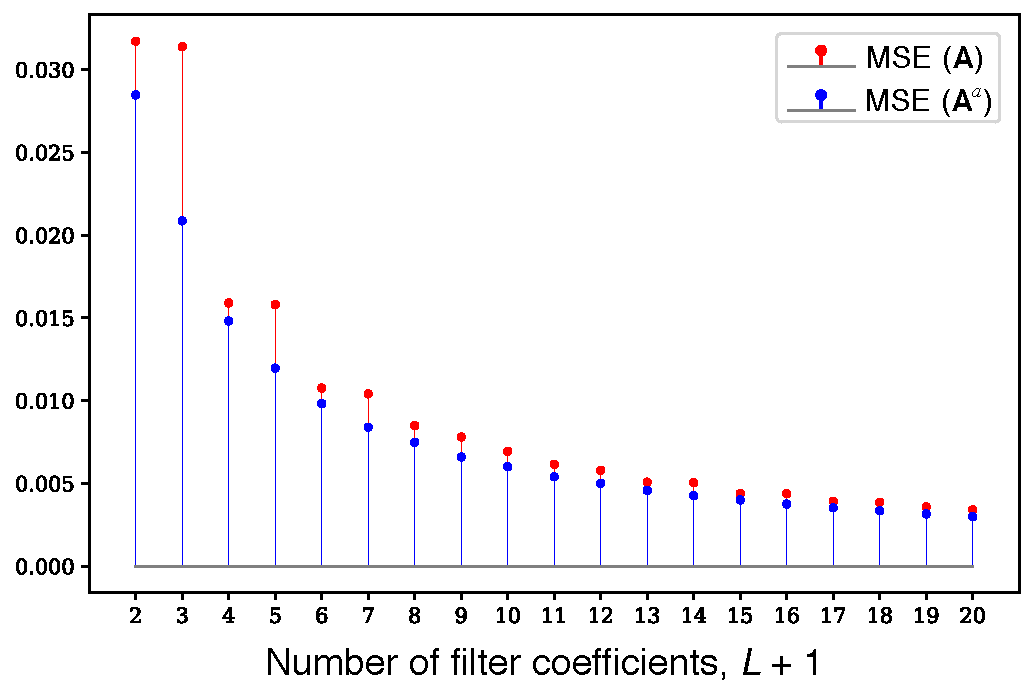
\includegraphics[width=0.65\linewidth]{Figures/ERROR_mse_min.pdf}
    \caption{Minimum approximation (mean squared) errors, for different values of $L$, between the ideal LPF and the filters designed by using the fractional graph shift operator $\mathbf{A}^a$ and the non-fractional operator $\mathbf{A}$.}%
    \label{fig:usa03}%
    %\vspace{-0.2cm}
\end{figure}

\begin{figure}[t!]
    \centering
    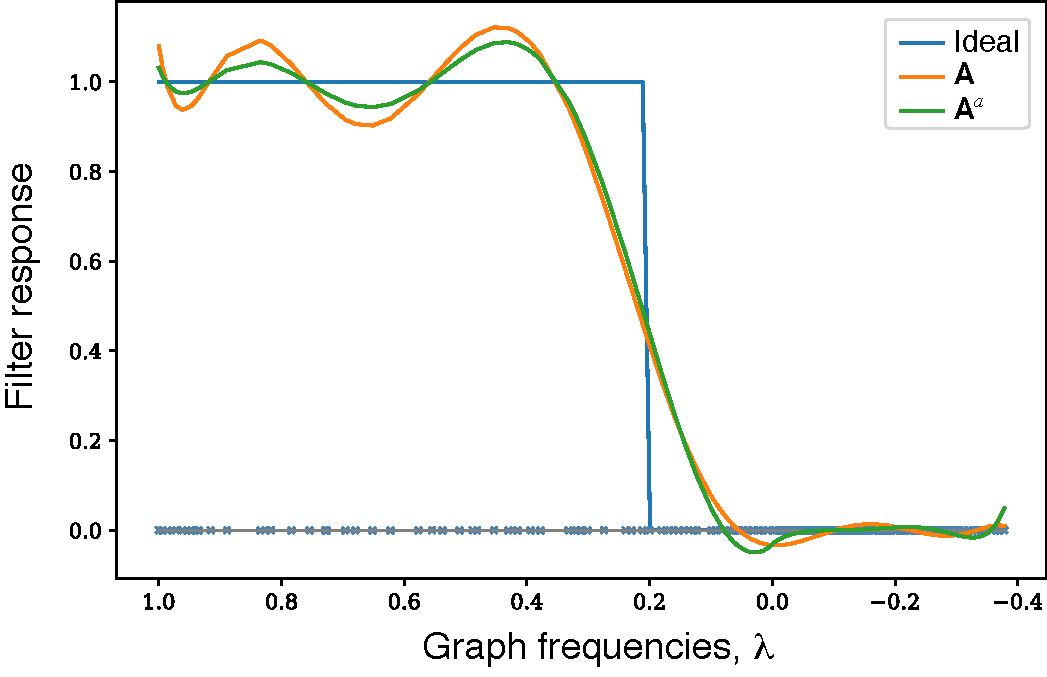
\includegraphics[width=0.65\linewidth]{Figures/ERROR_estacoes_resposta_grau10.pdf}%\vspace{-0.4cm}
    \caption{Ideal filter response superimposed on the responses obtained when $\mathbf{A}$ and $\mathbf{A}^a$, $a=0.855$, are used to design a filter with $L+1=10$ coefficients.}
    \label{fig:usa04}%
    %\vspace{-0.2cm}
\end{figure}

\subsection{Example: noise removal via LSI low-pass filtering}\label{subsec:lsi02}
In this example, we start from the same graph signal considered in Subsection~\ref{subsec:lsi01}. We add to the samples of the referred signal random uniformly-distributed values whose amplitude corresponds to a percentage of the range of the signal itself. Such a synthetic noise addition is intended to simulate what happens in many practical scenarios, in which measurements performed on a sensor network are subject to different sources of distortion. The resulting noisy signal is then filtered by the filters shown in Fig.~\ref{fig:usa04}, as an attempt to reduce the influence of the noise and recover the original signal.

During the experiment, the aforementioned percentage was varied from $1\%$ to $50\%$ and, for each of these values, $100$ noisy signals were generated. After low-pass filtering, the mean squared error between the original and filtered graph signals were computed. The results show that the filter designed using $\mathbf{A}^{0.855}$ allows to recover the signal with average reconstruction error always smaller than that with the filter designed using $\mathbf{A}$; see the data in Fig.~\ref{fig:usa05}.

{In this context, it is relevant to remark that the (best) fractional parameter $a=0.855$ has been found using the strategy described in the second paragraph of Subsection~\ref{subsec:lsi01}, which depends on the error between the designed filter and the ideal filter only. Therefore, the referred choice does not require prior knowledge of the original signal beforehand, which is usually not available in real-world problems.} This illustrates the potential gain that can be achieved, in this application scenario, when considering the possibility of fractionalization of the graph shift operator.

    {Finally, it is also interesting to mention that only one or a few nodes could have had their measurements corrupted by noise or changed due to other factors; this would represent, for instance, a scenario in which certain sensors would be malfunctioning. In order to obtain some preliminary results taking into account the above described assumption, additional simulations were carried out. The previous tests were repeated, but assuming that only a number from $1$ to $12$ nodes had their values nullified or increased by $20$ times. We then performed a low-pass filtering, expecting that the high-frequency component associated with the referred measurement changes would be attenuated and that the smooth behavior of the signal would be recovered. In general, the results obtained using the proposed fractional operator were better or at least equivalent to those obtained with the corresponding ordinary operator. Future works may address this issue in more detail.}

\begin{figure}[t!]
    \centering
    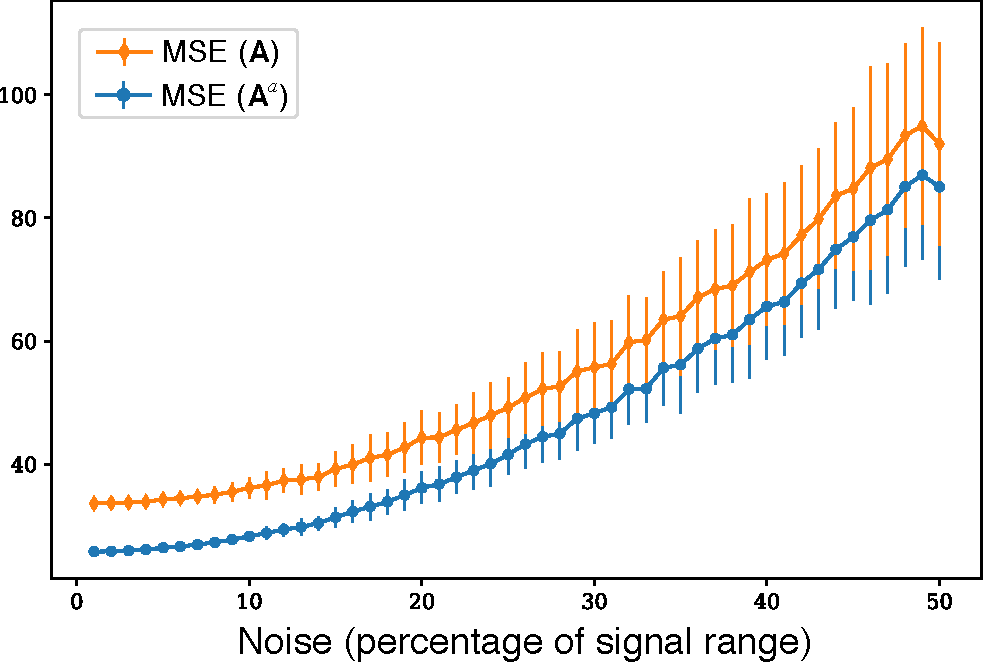
\includegraphics[width=0.7\linewidth]{Figures/ERROR_errobar_filtrados.pdf}
    \caption{Reconstruction (mean squared) errors after a noise removal procedure is performed by using graph filters with $L+1=10$ coefficients and designed from $\mathbf{A}$ and $\mathbf{A}^a$, $a=0.855$.}%
    \label{fig:usa05}%
    \vspace{-0.1cm}
\end{figure}

\section{Concluding remarks}\label{sec:conc}
This chapter proposed and discussed the fractional shift operator of graph signals. The core idea for the contribution was that, in the GSP theory, the unit shift is defined from the adjacency matrix of a graph. Interpreting the fractional shift as a filtering operation, it was demonstrated that, for ring graphs, its application produces the expected effect of approximating the classical ideal interpolating filter, exhibiting satisfactory results for bandlimited signals. Moreover, it was also shown that the referred fractional operator can be implemented as an LSI graph filter for arbitrary graphs and real-world examples were presented, illustrating the benefits of using $\mathbf{A}^a$ to design graph filters for noise removal.
